\documentclass[tikz,border=2pt]{standalone}
\usepackage{amsmath,amssymb}
\usepackage{tikz}
\usetikzlibrary{arrows.meta}

\begin{document}
% e^{x+iy} = e^x e^{iy}: a vertical line x = c in the z-plane is wrapped onto the circle of
% radius e^c, a horizontal line y = theta is sent onto the ray at angle theta.
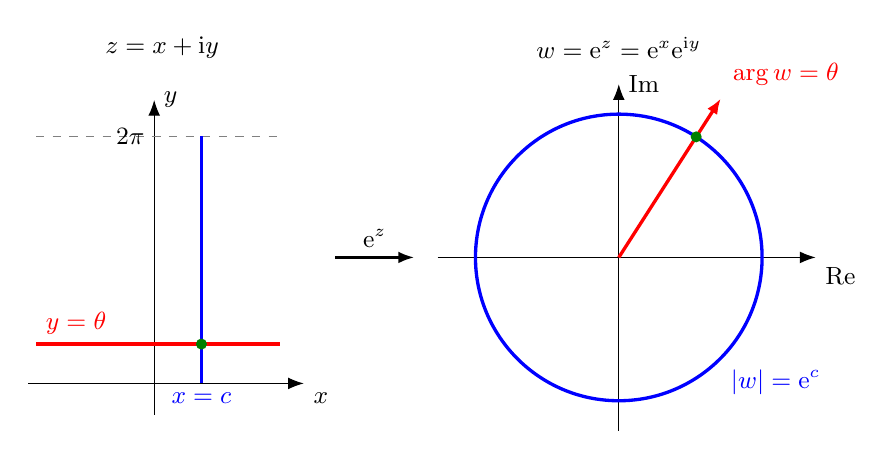
\begin{tikzpicture}[every node/.style={font=\small}, >={Latex[length=2mm]}]
	\draw[->] (-1.6,0) -- (1.9,0) node[below right] {$x$};
	\draw[->] (0,-0.4) -- (0,3.6) node[right] {$y$};
	\draw[gray, dashed] (-1.5,3.14) -- (1.6,3.14);
	\draw[blue, very thick] (0.6,0) -- (0.6,3.14);
	\draw[red, very thick] (-1.5,0.5) -- (1.6,0.5);
	\node[blue, font=\small, below] at (0.6,0) {$x=c$};
	\node[red, anchor=south west] at (-1.5,0.5) {$y=\theta$};
	\fill[green!50!black] (0.6,0.5) circle (2pt);
	\node[font=\small, left] at (0,3.14) {$2\pi$};
	\node[anchor=south] at (0.1,4.0) {$z=x+\mathrm{i}y$};
	\draw[->, thick] (2.3,1.6) -- (3.3,1.6) node[midway, above] {$\mathrm{e}^{z}$};
	\begin{scope}[xshift=5.9cm, yshift=1.6cm]
		\draw[->] (-2.3,0) -- (2.5,0) node[below right] {$\mathrm{Re}$};
		\draw[->] (0,-2.2) -- (0,2.2) node[right] {$\mathrm{Im}$};
		\draw[blue, very thick] (0,0) circle (1.82);
		\draw[red, very thick, ->] (0,0) -- (57.3:2.4);
		\node[blue, font=\small, anchor=north west] at (1.3,-1.3) {$|w|=\mathrm{e}^{c}$};
		\node[red, font=\small, anchor=south west] at (57.3:2.45) {$\arg w=\theta$};
		\fill[green!50!black] (57.3:1.82) circle (2pt);
		\node[anchor=south] at (0,2.4) {$w=\mathrm{e}^{z}=\mathrm{e}^{x}\mathrm{e}^{\mathrm{i}y}$};
	\end{scope}
\end{tikzpicture}
\end{document}
